%% --------------------------------------------------------------
%%
%% A F T E R G L O W
%%
%% --------------------------------------------------------------
\begin{frame}%{Afterglow}
\begin{tikzpicture}[overlay,remember picture]
\uncover<1->{ % <-> |
    \node (t1) [anchor=center,scale=1,opacity=1] at ([shift={(-0.8cm,2.2cm)}]current page.center){
        \parbox{0.95\textwidth}{
            \begin{footnotesize}
                \textbf{Afterglow} non-thermal (synchrotron) emission arasing from ejecta moving through ISM\footcite{Sari:1997qe,Kumar:2014upa};
            \end{footnotesize}
            \begin{itemize}
                \item Long \ac{GRB} (associated with supernovae)
                \item Short \ac{GRB} (predicted to occure at \ac{BNS} mergers)
            \end{itemize}
            \textbf{Kilonova afterglow} -- expected\footcite{Nakar:2011cw,Kathirgamaraju:2019xwu}, but no clear detection
%            \begin{itemize}
%                \item Ejecta moves through ISM $\rightarrow$ synchrotron emission (afterglow)\footcite{Sari:1997qe,Kumar:2014upa}%$^{\textcolor{gray}{\text{\cite{Sari:1997qe}}}}$
%                \item \GRB{} afterglow, structured jet, off-axis\footcite{Hajela:2019mjy}%$^{\textcolor{gray}{\text{\cite{Hajela:2019mjy}}}}$
%                \item expected kN ejecta afterglow\footcite{Kathirgamaraju:2019xwu}%$^{\textcolor{gray}{\text{\cite{Kathirgamaraju:2019xwu}}}}$
%            \end{itemize}
    }};
}

\uncover<2->{ % <-> |
    \node (t1) [anchor=center,scale=1,opacity=1] at ([shift={(-3.5cm,-0.2cm)}]current page.center){
        \parbox{0.60\textwidth}{
            \textbf{\GRB{}:} counterpart to \GW{} -- structured jet, observed off-axis\footcite{Troja:2017nqp,Hajela:2019mjy}\\
            \textbf{Rebrightening} $1243$~days post-merger\footcite{Hajela:2021faz};
    }};
}

%\uncover<1->{ % <-> |
%    \node (t1) [anchor=center,scale=1,opacity=1] at ([shift={(-3.5cm,-2.0cm)}]current page.center){
%        \parbox{0.60\textwidth}{
%            \textbf{Rebrightening} $1243$~days post-merger\footcite{Hajela:2021faz};
%            \begin{itemize}
%                \item change in microphysics parameters;
%                \item ISM density variation;
%                \item emergence of a new component;
%            \end{itemize}
%    }};
%}

\uncover<3->{ % <-> |
    \node (t1) [anchor=center,scale=1,opacity=1] at ([shift={(-3.5cm,-2.0cm)}]current page.center){
        \parbox{0.60\textwidth}{
            \textbf{Question:} can kilonova afterglow explain observations?
%            \begin{itemize}
%                \item change in microphysics parameters;
%                \item ISM density variation;
%                \item emergence of a new component;
%            \end{itemize}
    }};
}

%\uncover<1->{ % <-> |
%    \node (t1) [anchor=center,scale=1,opacity=1] at ([shift={(5.0cm,1.8cm)}]current page.center){
%        \parbox{0.40\textwidth}{
%            \textbf{ Light curve peak$^{\textcolor{gray}{\text{\cite{Nakar:2019fza}}}}$: }
%            \begin{equation*}
%                \begin{aligned}
%                    F_{\nu,p} & \propto E n^{(p+1)/4}  
%                    \textcolor{black}{ \beta^{(5p-7)/2} }   \\
%                    & \times \varepsilon_e^{p-1}\varepsilon_B^{(p+1)/4} D_L^{-2}\nu^{(-p-1)/2} \\
%                    t_{p} & \propto E^{1/3} n^{-1/3} 
%                    \textcolor{black}{ \beta^{-5/3} }
%                \end{aligned}
%            \end{equation*}
%    }};
%}

\uncover<1->{ % <-> |
    \node (img1) [anchor=center,scale=1,opacity=1] at ([shift={(5.2cm,-1.8cm)}]current page.center){
        \parbox{0.5\textwidth}{
            %\includegraphics[height=6.3cm]{phd_figs/jet_ascenci20.pdf}
            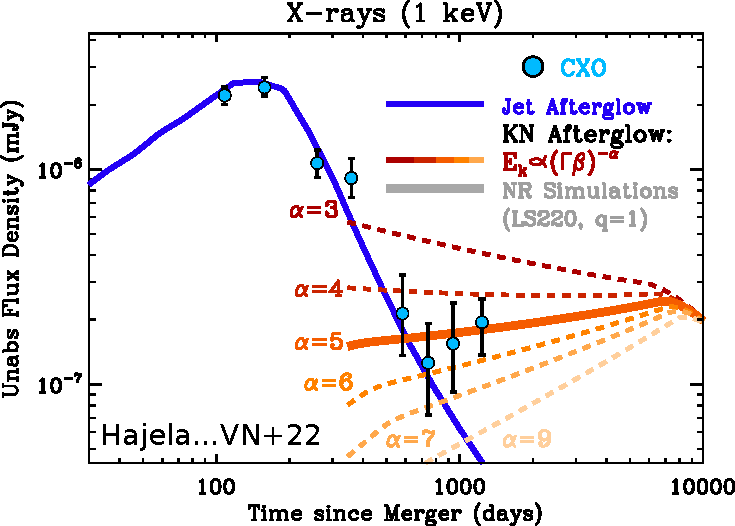
\includegraphics[height=4.5cm]{figures/Hajela22_obs_pl_noNR.pdf}
            %Artist depiction of ejecta$^\text{\citep{Ascenzi:2020xqi}}$
    }};
}



\end{tikzpicture}
\end{frame}

%% =======================================================
%%
%%                   Method
%%
%% =======================================================

%\begin{frame}{Method} %% ---------- title 
%
%\begin{tikzpicture}[overlay,remember picture]
%
%\uncover<1->{ % <-> |
%    \node (t1) [anchor=center,scale=1,opacity=1] at ([shift={(-3.9cm,-0.7cm)}]current page.center){
%        \parbox{0.53\textwidth}{
%            Passing through the cold ISM, shock front 
%            \begin{itemize}
%                \item randomizes the particles' $\vec{\upsilon}$,
%                \item compresses the plasma,
%                \item amplifies the magnetic fields 
%                \item accelerates the inbound particles % to a power-law distribution function.
%            \end{itemize}
%            
%            \textbf{Dynamics} --
%            %A relativistic shock propagating into a cold upstream medium.
%            $3$ conservation laws: baryon number, energy, momentum fluxes across shock front.
%%            The latter two $T^{\mu\nu} = (\rho' c^2 + p') u^{\mu} u^{\nu} + p' g^{\mu\nu},$
%            %
%%            These equations can be written as 
%            %
%%            \begin{equation} % subequations
%%            \begin{aligned} % align
%%            \frac{e_2'}{n_2'} &= (\gamma_{21} - 1)m_p c^2 \\
%%            \frac{n_2'}{n_1'} &= \frac{\hat{\gamma}\gamma_{21} + 1}{\hat{\gamma}-1} \\
%%            \gamma_{1s}^2 &= \frac{(\gamma_{21} + 1) [\hat{\gamma}(\gamma_{21}-1)+1]^2}{\hat{\gamma}(2-\hat{\gamma})(\gamma_{21}-1)+2}
%%            \end{aligned} % align
%%            \label{eq:afterglow:blast}
%%            \end{equation} % subequations
%            %
%%            \begin{figure*}[t]
%%            \centering 
%%            \includegraphics[width=0.45\textwidth]{Fig_8_KZ.pdf}
%%            \caption{
%%                This is a schematic sketch of a pair of shocks produced when a relativistic
%%                jet from a \ac{GRB} collides with the \ac{CBM}, as viewed from the
%%                rest frame of unshocked \ac{CBM}. Regions 2 \& 3 represent shocked \ac{CBM} and \ac{GRB}
%%                jet respectively. They move together with the same \ac{LF} ($\gamma_2$, as viewed
%%                by a stationary observer in the unshocked \ac{CBM}), and have the same pressure but
%%                different densities.
%%                (Adapted from \citet{Kumar:2014upa}, figure~8)
%%            }
%%            \label{fig:aafg:theory:sr8}
%%            \end{figure*}
%            %
%%            where subscripts $2$ and $1$ stand for downstream and upstream respectively, 
%%            $e'$ is the internal energy density, $n'$ is the proton number density, 
%%            $\gamma_{21}$ is the relative \ac{LF} of plasma in region 
%%            $2$ with respect to the region $1$
%%            $\gamma_{1s}$ is the relative \ac{LF} of plasma in region $1$ with respect to the shock front,
%%            $\hat{\gamma}$ is the adiabatic index of the fluid, for the ideal, relativistic 
%%            fluid is $\hat{\gamma}=4/3$ and subrelativisitc $\hat{\gamma}=5/3$.
%%            The $2$ and $1$ regions are also shown in Fig.~\ref{fig:aafg:theory:sr8} 
%%            (see also \cite{Nava:2013} for a more comprehensive take).
%%            %
%%            Solving the system Eq.~\eqref{eq:afterglow:blast} gives the full evolution 
%%            of the \blast{}. 
%            
%            \textbf{Electrons:} continuity eq. in energy space 
%            \begin{equation*}
%            \frac{\partial }{\partial t}\frac{d n_e}{d\gamma_e} + \frac{\partial}{\partial \gamma_e}\Big[ \dot{\gamma_e}\frac{dn_e}{d\gamma_e} \Big] = S(\gamma_e), \rightarrow \frac{d n_e}{d\gamma_e} \propto \gamma^{-p}
%            \end{equation*}
%            %
%            Charactersitc, $\gamma_c$ , $\gamma_M$ , $\gamma_m$
%            %
%%            where $\dot{\gamma_e} = -\sigma_T B^2 \gamma_e^2 / (6\pi m_e c)$ is the rate at 
%%            which electron \ac{LF} changes due to losses, $S(\gamma_e)$ is the injection 
%%            rate of electrons into the system.
%%            %
%%            Assume that the minimum \ac{LF} of injected electrons is $\gamma_m$, \eg, 
%%            where $S(\gamma_e) = 0$ for $\gamma_e < \gamma_m$.
%%            %
%%            \begin{equation}
%%            dn_e/d\gamma_e \propto 
%%            \begin{cases}
%%            \gamma_e^{-2} &\text{ if } \gamma_c < \gamma_e < \gamma_m, \\
%%            \gamma_e^{-p-1} &\text{ if } \gamma_e > \gamma_c > \gamma_m
%%            \end{cases}
%%            \label{eq:afterglow:elec_dist}
%%            \end{equation}
%            
%    }};
%
%    \node (t2) [anchor=center,scale=1,opacity=1] at ([shift={(3.9cm,-0.7cm)}]current page.center){
%    \parbox{0.53\textwidth}{
%        \textbf{Synchrotron emission} %\citep{RybickiLightman:1985} --
%        %
%        \begin{equation*}
%        P_{syn} = \frac{2q^4 E^2}{3c^3 m_e^2}
%        \,
%        \omega_{syn}\sim\frac{qB\gamma_e^2}{m_e c}
%        %\,
%        %P_{syn}(\nu_{syn}) \sim P_{syn}/\nu_{syn}
%        \end{equation*}
%        %
%        \begin{equation*}
%        f_{\nu} = \int_{\gamma_{\nu}}^{\infty} d\gamma_e \frac{dn_e}{d\gamma_e}P_{syn}(\nu) 
%        \end{equation*}
%        
%        \textbf{EATS}
%        %
%        \begin{equation*}
%        F(\nu,t) = c\int_0^{\theta}\int_{0}^{r}\frac{P'(\nu',t_{em},r)}{\Gamma^2(1-\beta\cos\theta)^2}r^2 dr d\cos\theta
%        \end{equation*}
%        with $c = (1+z) / (2d_L^2)$
%}};
%}
%\end{tikzpicture}
%\end{frame}
\begin{frame}{Dynamics}  %% ---------- Intro/motivation 
    \begin{tikzpicture}[overlay,remember picture]
        \uncover<1->{ % <-> |
            \node (t1) [anchor=center,scale=1,opacity=1] at ([shift={(-0.6cm,-0.0cm)}]current page.center){
                \parbox{1.\textwidth}{
                    Semi-analytic model (energy conservation) in a 
                    this-shel approximation; \\
                    
                    %From stress-energy tensor %$ T^{\mu\nu} = (\rho' c^2 + p') u^{\mu}u^{\nu} + p' g^{\mu\nu}$ \\
                    %we write evolution equation: 
                    \vspace{-2mm}
                    \begin{equation*}
                        \begin{aligned}
                            dE_{\rm tot} = 0 \rightarrow & d [ \Gamma (M_0 + m) c^2 + \Gamma_{\rm eff}E_{\rm int}' ] = dm c^2 + \Gamma_{\rm eff} dE_{\rm rad}'. \\
                            & dE_{\rm int}' = dE_{\rm sh}' + dE_{\rm ad}' + dE_{\rm rad}',
                        \end{aligned}
                    \end{equation*}
                    
                    Adiabatic evolution, $d\Gamma/dR$; \\
                    If $\rho_{\rm ISM}=\text{const}$: free-coasting ($\Gamma=\Gamma_0$), and deceleration $\Gamma\downarrow$.\\
                    
                    \textbf{Structure:} lateral, $\{\theta_i\}$, and velocity $\{\upsilon_i\}$; \\
                    \textbf{Initial conditions}: ejecta profile, \\
                    $\{ E_{ij, 0} \}=f(\Gamma_{i, 0},\theta_{j, 0})$; %($\Gamma=(1-\beta^2)^{-2}$); $\beta=\upsilon/c$; \\
                    %\textbf{Main stages:} free-coasting + deceleration; \\
                    %$\Gamma$ is the bulk Lorentz factor. \\
                    %\textbf{Shock properties}, $\rho_{\rm sh}$, $\beta_{\rm sh}$, $R_{\rm sh}$ \\
            }};
            
        }
%        \uncover<1->{ % <-> |
%            \node (t1) [anchor=center,scale=1,opacity=1] at ([shift={(4.0cm,-2.0cm)}]current page.center){
%                \parbox{0.5\textwidth}{
%                    \textbf{Evolution}: free-coasting + deceleration; \\
%                    %Electrons accelerated to power-law distribution $\gamma_e^{-p}$
%                    Total energy in electrons and magnetic fields $\epsilon_e$, $\epsilon_B$;
%                    Assume for electrons local istropic distribution of angles relative $\vec{B}$; \\
%                    Assume $\vec{B}$ is random mix of orientations; \\
%                    Spectrum from a PL electrons is also PL; \\
%                    %Assume local cooling rate $=$ expansion time
%                    Emission is isotropic in the rest-frame
%                    %Intensity-weighted mean change in any charactersitic gets broadened
%            }};
%        }
        % Margalit B., Quataert E., 2021, ApJL, 923, L14. 
%        \uncover<1->{ % <-> |
%            \node (t1) [anchor=center,scale=1,opacity=1] at ([shift={(-4.4cm,-2.4cm)}]current page.center){
%                \parbox{0.5\textwidth}{
%                    \begin{equation*}
%                        P_{\nu'} = \int_{\gamma_{\nu'}}^{\infty} d\gamma_e \frac{dn'}{d\gamma_e}P_{s}'(\nu'); \hspace{3mm} \frac{dn'}{d\gamma_e} \propto
%                        \begin{cases}
%                            \gamma_e^{-2} &\text{s.c.} \\ 
%                            \gamma_e^{-p-1} &\text{f.c.}
%                        \end{cases}
%                    \end{equation*}
%                    %
%                    \begin{equation*}
%                        F(\nu,t) = \frac{1+z} {2d_L^2}\int_0^{\theta}\int_{0}^{r}\frac{P'(\nu',t_{\rm em},r)}{\Gamma^2(1-\beta\cos\theta)^2}r^2 dr d\cos\theta
%                    \end{equation*}
%                    \textbf{Synchrotron Radiation}
%            }};
%        }
        
        %        \uncover<1-1>{ % <-> |
            %            \node (img1) [anchor=center,scale=1,opacity=1] at ([shift={(4.5cm,-0.3cm)}]current page.center){
                %                \parbox{0.6\textwidth}{
                    %                    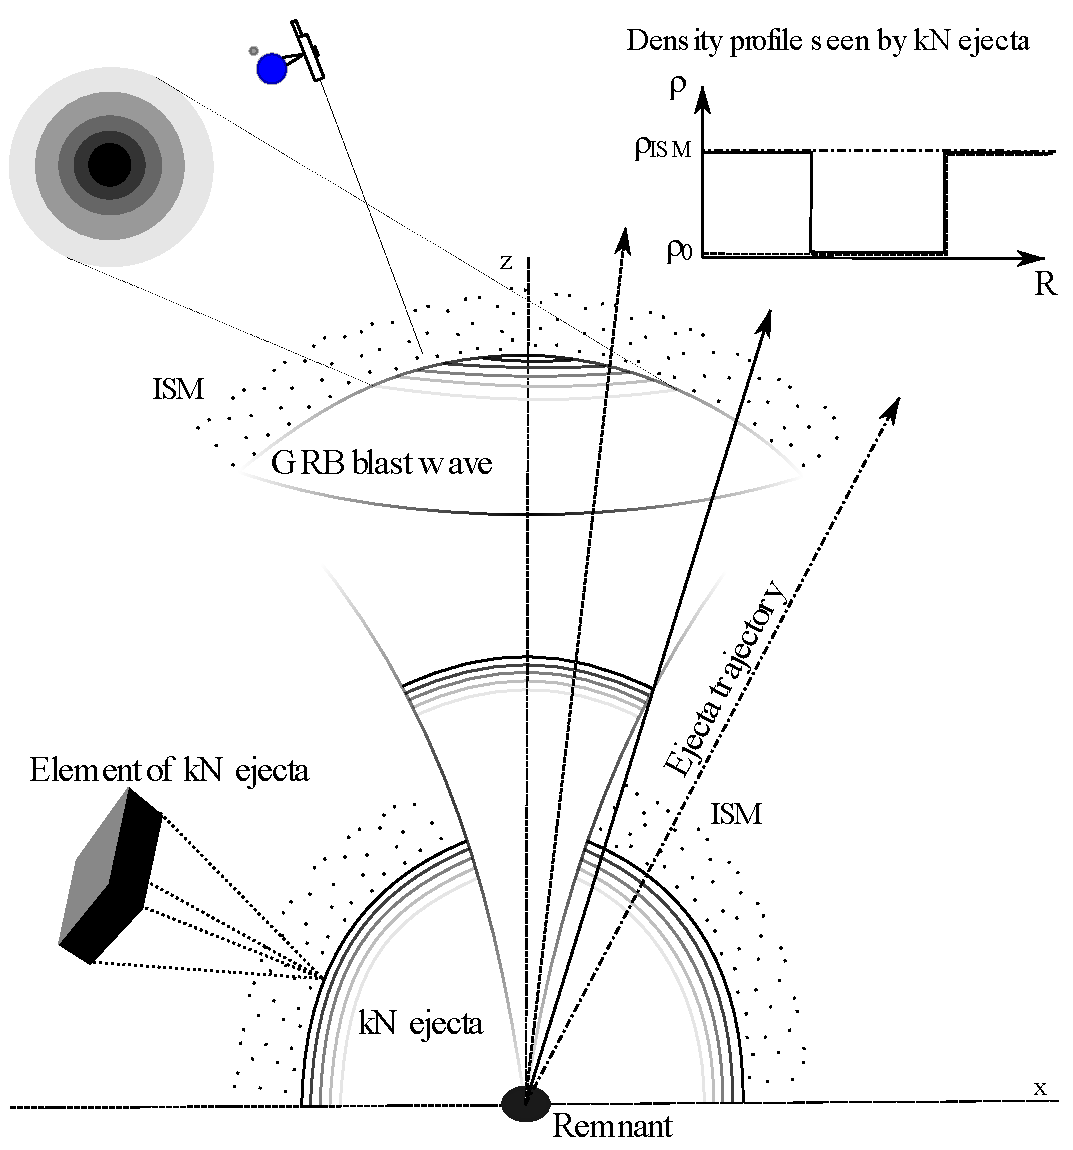
\includegraphics[height=7.8cm]{figures/structure2.pdf}
                    %                    %\includesvg[height=7.2cm]{figures/structure2}
                    %            }};
            %        }
                \uncover<1->{ % <-> |
                        \node (img1) [anchor=center,scale=1,opacity=1] at ([shift={(5.0cm,-2.4cm)}]current page.center){
                                \parbox{0.6\textwidth}{
                                        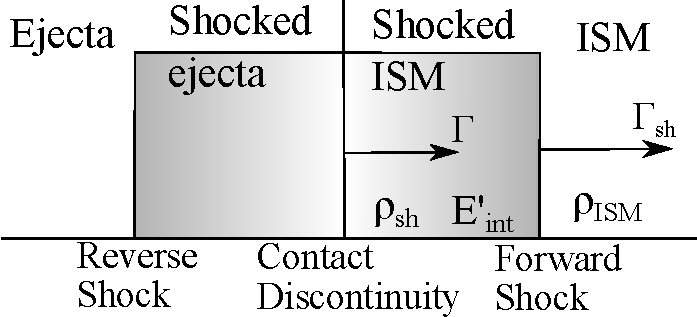
\includegraphics[height=3.0cm]{figures/shock_scatch2.pdf}
                                }};
                        
                    }
        
    \end{tikzpicture}
\end{frame}

%\begin{frame}{Radiation}  %% ---------- Intro/motivation 
%    \begin{tikzpicture}[overlay,remember picture]
%        \uncover<1->{ % <-> |
%            \node (t1) [anchor=center,scale=1,opacity=1] at ([shift={(-3.6cm,1.4cm)}]current page.center){
%                \parbox{0.6\textwidth}{
%                    \textbf{A shock}\footcite{Zhang:2018book}%$^{\textcolor{gray}{\text{\cite{Rezzolla:2013,Kumar:2014upa,Zhang:2018book,Nava:2013}}}}$
%                    \begin{itemize}
%                        \item comresses fluid, $\rho_{\rm sh} = 4 \Gamma_{\rm sh} \rho_{\rm ISM}$
%                        \item amplifies magnetic fields, $B=\sqrt{8 \pi \epsilon_B e'}$
%                        \item accelerates electrons, $\frac{dn'}{d\gamma_e} \propto \gamma_e^{-p}$ 
%                    \end{itemize}
%                    
%            }};
%            
%        }
%        \uncover<1->{ % <-> |
%            \node (t1) [anchor=center,scale=1,opacity=1] at ([shift={(4.6cm,1.3cm)}]current page.center){
%                \parbox{0.6\textwidth}{
%                    \textbf{Electron spectrum}$^{\textcolor{gray}{\text{\cite{Sari:1997qe}}}}$ \\
%                    Broken power law (BPL) with 
%                    \vspace{-3mm}
%                    \begin{equation*}\label{eq:method:gm_pl_only}
%                        \gamma_m' = \frac{p-2}{p-1} \frac{\epsilon_e e'}{n' m_e c^2} \hspace{3mm} 
%                        \gamma_c' = \frac{6 \pi m_e c \Gamma}{\sigma_T t_{\rm em} B'^2}, \hspace{3mm}
%                        %e' = \frac{E_{\rm int}'}{V'}
%                    \end{equation*}
%                    Regimes: $\gamma_m' < \gamma_c' (>\gamma_c')$: slow (fast) cooling
%            }};
%            
%        }
%%        \uncover<1->{ % <-> |
%%            \node (t1) [anchor=center,scale=1,opacity=1] at ([shift={(4.0cm,-2.0cm)}]current page.center){
%%                \parbox{0.5\textwidth}{
%%                    \textbf{Evolution}: free-coasting + deceleration; \\
%%                    %Electrons accelerated to power-law distribution $\gamma_e^{-p}$
%%                    Total energy in electrons and magnetic fields $\epsilon_e$, $\epsilon_B$;
%%                    Assume for electrons local istropic distribution of angles relative $\vec{B}$; \\
%%                    Assume $\vec{B}$ is random mix of orientations; \\
%%                    Spectrum from a PL electrons is also PL; \\
%%                    %Assume local cooling rate $=$ expansion time
%%                    Emission is isotropic in the rest-frame
%%                    %Intensity-weighted mean change in any charactersitic gets broadened
%%            }};
%%        }
%        % Margalit B., Quataert E., 2021, ApJL, 923, L14. 
%        \uncover<1->{ % <-> |
%            \node (t1) [anchor=center,scale=1,opacity=1] at ([shift={(-4.4cm,-2.2cm)}]current page.center){
%                \parbox{0.5\textwidth}{
%                    \textbf{Synchrotron Radiation$^{\textcolor{gray}{\text{\cite{RybickiLightman:1985,Sari:1997qe,Johannesson:2006zs}}}}$}
%%                    \begin{equation*}
%%                        P_{\nu'} =  \int_{\gamma_{\nu'}}^{\infty} d\gamma_e \frac{dn'}{d\gamma_e}p'(\nu'), \hspace{2mm}
%%                        p'(\nu')=\frac{\sigma_T B^2 \gamma_e \upsilon_e^2}{4\pi c};
%%%                        \hspace{3mm} \frac{dn'}{d\gamma_e} \propto
%%%                        \begin{cases}
%%%                            \gamma_e^{-2} &\text{s.c.} \\ 
%%%                            \gamma_e^{-p-1} &\text{f.c.}
%%%                        \end{cases}
%%                    \end{equation*}
%                    \begin{equation*}
%                        P_{\nu'}' =  \text{BPL}\big(\nu',\, \nu_m'(\gamma_m'),\, \nu_c'(\gamma_c')\big)
%                    \end{equation*}
%                    \textbf{Observed flux density$^{\textcolor{gray}{\text{\cite{Granot:2005cc}}}}$}
%                    \begin{equation*}
%                        F(\nu,t) = \frac{1+z} {2d_L^2}\int_0^{\theta}\int_{0}^{r}\frac{P'(\nu',t_{\rm em},r)}{\Gamma^2(1-\beta\cos\theta)^2}r^2 dr d\cos\theta
%                    \end{equation*}
%            }};
%        }
%        
%        %        \uncover<1-1>{ % <-> |
%            %            \node (img1) [anchor=center,scale=1,opacity=1] at ([shift={(4.5cm,-0.3cm)}]current page.center){
%                %                \parbox{0.6\textwidth}{
%                    %                    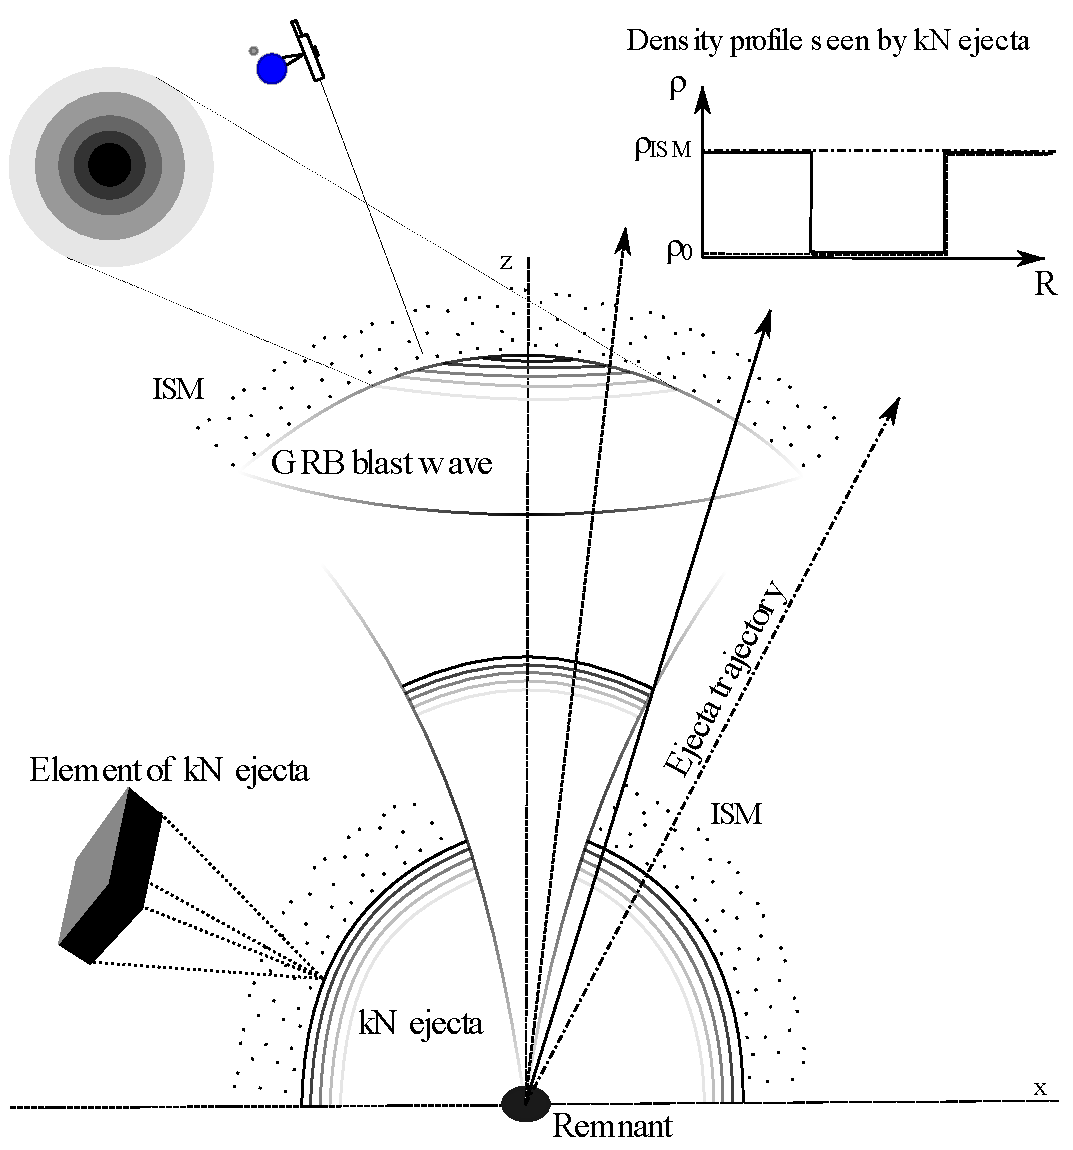
\includegraphics[height=7.8cm]{figures/structure2.pdf}
%                    %                    %\includesvg[height=7.2cm]{figures/structure2}
%                    %            }};
%            %        }
%        %        \uncover<1->{ % <-> |
%            %            \node (img1) [anchor=center,scale=1,opacity=1] at ([shift={(-0.0cm,-2.4cm)}]current page.center){
%                %                \parbox{1.0\textwidth}{
%                    %                    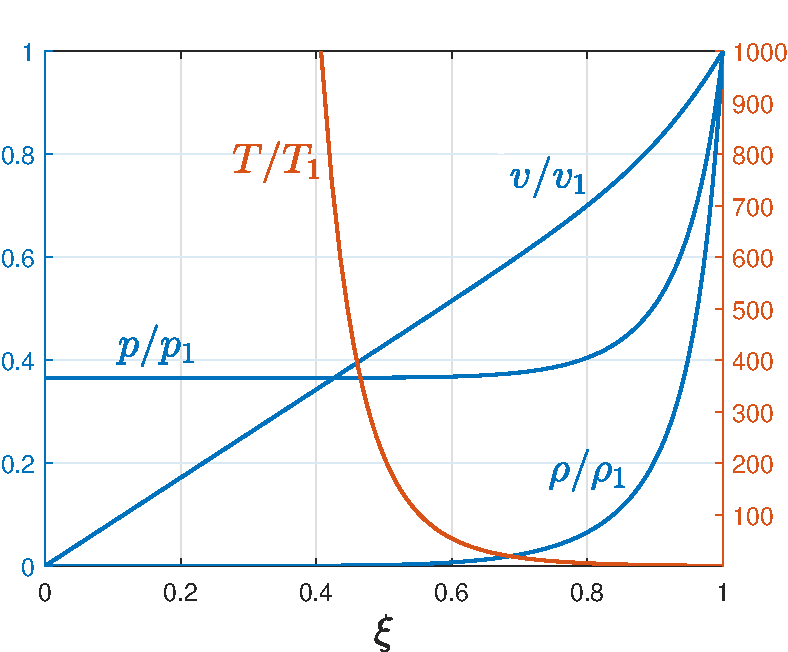
\includegraphics[height=3.5cm]{figures/TNS_blast_wave.pdf}
%                    %            }};
%            %            
%            %        }
%        \uncover<1->{ % <-> |
%            \node (img1) [anchor=center,scale=1,opacity=1] at ([shift={(4.8cm,-2.2cm)}]current page.center){
%                \parbox{0.6\textwidth}{
%                        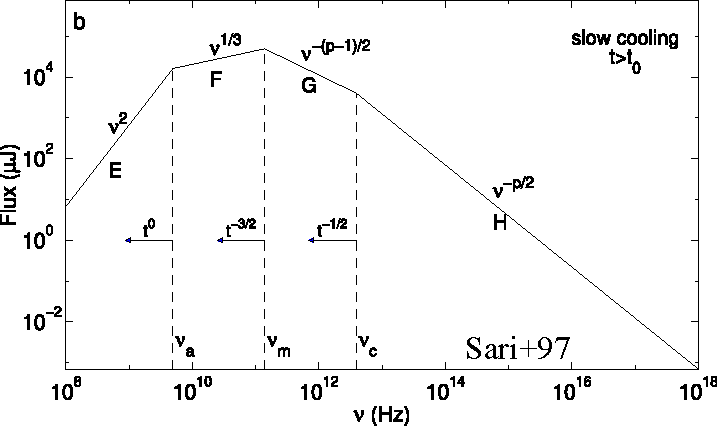
\includegraphics[height=4.0cm]{figures/Sari97_spectrum_slow_cool.pdf}
%%                        Overall, an afterglow spectrum has three characteristic frequencies: 
%%                        (i) $\nu_i$ (injection break) at which most of the injected electrons radiate 
%%                        (ii) $\nu_c$ (cooling break) at which for electrons expansion timescale is equal 
%%                        to the radiative cooling timesacle
%%                        (iii) $\nu_a$ an absorption break, below which synchrotron emission is absorbed by 
%%                        electrons in free-free transitions in magnetic fields, (\ac{SSA}).
%            }};
%        }
%    \end{tikzpicture}
%\end{frame}
\begin{frame}{Radiation}  %% ---------- Intro/motivation 
    \begin{tikzpicture}[overlay,remember picture]
        \uncover<1->{ % <-> |
            \node (t1) [anchor=center,scale=1,opacity=1] at ([shift={(-3.6cm,1.4cm)}]current page.center){
                \parbox{0.6\textwidth}{
                    \textbf{A shock}\footcite{Zhang:2018book}%$^{\textcolor{gray}{\text{\cite{Rezzolla:2013,Kumar:2014upa,Zhang:2018book,Nava:2013}}}}$
                    \begin{itemize}
                        \item comresses fluid, $\rho_{\rm sh} = 4 \Gamma_{\rm sh} \rho_{\rm ISM}$
                        \item amplifies magnetic fields, $B=\sqrt{8 \pi \epsilon_B e'}$
                        \item accelerates electrons, $\frac{dn'}{d\gamma_e} \propto \gamma_e^{-p}$ 
                    \end{itemize}
                    
            }};
            
        }
        \uncover<1->{ % <-> |
            \node (t1) [anchor=center,scale=1,opacity=1] at ([shift={(4.6cm,1.3cm)}]current page.center){
                \parbox{0.6\textwidth}{
                    \textbf{Synchrotron radiation spectrum}\footcite{Sari:1997qe,Wijers:1998st} \\%$^{\textcolor{gray}{\text{\cite{Sari:1997qe}}}}$ \\
                    Broken power law (BPL); \\ 
                    $\nu_m\propto\gamma_m$, $\nu_c\propto\gamma_c$ \\
            }};
            
        }

        \uncover<1->{ % <-> |
            \node (t1) [anchor=center,scale=1,opacity=1] at ([shift={(-4.4cm,-1.7cm)}]current page.center){
                \parbox{0.5\textwidth}{
                    \textbf{Electron spectrum}: %$^{\textcolor{gray}{\text{\cite{Sari:1997qe}}}}$ \\
                    broken power law (BPL) with 
                    \vspace{-3mm}
                    \begin{equation*}\label{eq:method:gm_pl_only}
                        \gamma_m' = \frac{p-2}{p-1} \frac{\epsilon_e e'}{n' m_e c^2} \hspace{3mm} 
                        \gamma_c' = \frac{6 \pi m_e c \Gamma}{\sigma_T t_{\rm em} B'^2}, \hspace{3mm}
                        %e' = \frac{E_{\rm int}'}{V'}
                    \end{equation*}
                \vspace{-5mm}
                    \begin{footnotesize}
                        \begin{itemize}
                            \item Slow cooling $\gamma_m' < \gamma_c'$
                            \item Fast cooling $\gamma_m' > \gamma_c'$
                        \end{itemize}
                    \end{footnotesize}
            }};
        }

        \uncover<1->{ % <-> |
            \node (img1) [anchor=center,scale=1,opacity=1] at ([shift={(4.5cm,-1.9cm)}]current page.center){
                \parbox{0.6\textwidth}{
                    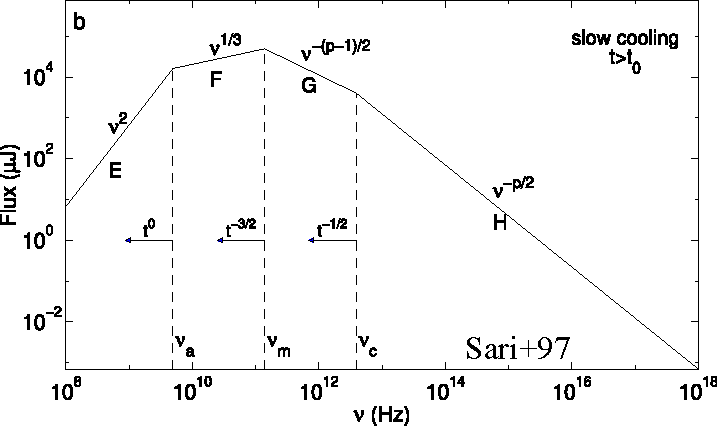
\includegraphics[height=4.5cm]{figures/Sari97_spectrum_slow_cool.pdf}
                    %                        Overall, an afterglow spectrum has three characteristic frequencies: 
                    %                        (i) $\nu_i$ (injection break) at which most of the injected electrons radiate 
                    %                        (ii) $\nu_c$ (cooling break) at which for electrons expansion timescale is equal 
                    %                        to the radiative cooling timesacle
                    %                        (iii) $\nu_a$ an absorption break, below which synchrotron emission is absorbed by 
                    %                        electrons in free-free transitions in magnetic fields, (\ac{SSA}).
            }};
        }
    \end{tikzpicture}
\end{frame}
%% =======================================================
%%
%%                   Method :: Code
%%
%% =======================================================

%\begin{frame}{Method :: \texttt{PyBlastAfterglow}} %% ---------- title 
%
%\begin{tikzpicture}[overlay,remember picture]
%
%\uncover<1->{ % <-> |
%    \node (t1) [anchor=center,scale=1,opacity=1] at ([shift={(-3.9cm,-0.7cm)}]current page.center){
%        \parbox{0.53\textwidth}{
%            \textbf{Blast wave dynamics} 
%            \begin{itemize}
%                \item[\textcolor{black}{$\blacksquare$}] uniform ISM; FS only$^\text{\citep{Peer:2012}}$
%                \item[\textcolor{blue}{$\blacksquare$}] $\forall$ ISM, FS/RS; Rad.Loss$^\text{\citep{Nava:2013}}$
%            \end{itemize}
%            \textbf{Transrelativisitc Equation of state}
%            \begin{itemize}
%                \item[\textcolor{black}{$\blacksquare$}]Assymptic$^\text{\citep{Nava:2013}}$
%                \item[\textcolor{blue}{$\blacksquare$}] HD-simulation informed$^\text{\citep{Peer:2012}}$
%            \end{itemize}
%            \textbf{Lateral Spreading}
%            \begin{itemize}
%                \item[\textcolor{black}{$\blacksquare$}] Speed of sound limited$^\text{\citep{Huang:1999di}}$
%                \item[\textcolor{blue}{$\blacksquare$}] 2D HD -informed$^\text{\citep{Granot:2012}}$ 
%            \end{itemize}
%    }};
%}
%
%\uncover<1->{ % <-> |
%    \node (t2) [anchor=center,scale=1,opacity=1] at ([shift={(3.9cm,-0.7cm)}]current page.center){
%        \parbox{0.53\textwidth}{
%            \textbf{Electron distribution} 
%            \begin{itemize}
%                \item[\textcolor{black}{$\blacksquare$}] Simple 2-segment \ac{BPL}
%                \item[\textcolor{blue}{$\blacksquare$}] \ac{BPL} with accurate crit. Lorentz. Fact.
%                \item[\textcolor{gray}{$\blacksquare$}] $\forall$ segmented electron distribution
%            \end{itemize}
%            \textbf{Synchrotron spectrum}
%            \begin{itemize}
%                \item[\textcolor{black}{$\blacksquare$}] 3-segment \ac{BPL} $^\text{\citep{Sari:1997qe}}$
%                \item[\textcolor{blue}{$\blacksquare$}] Smooth \ac{BPL}$^\text{\citep{Johannesson:2006zs}}$ + SSA$^\text{\citep{Johannesson:2018cdl}}$
%                \item[\textcolor{gray}{$\blacksquare$}] Direct integration of syntronton function$^\text{\citep{Dermer:2009}}$
%            \end{itemize}
%            \textbf{Equal time arrival surface integrator}
%            \begin{itemize}
%                \item[\textcolor{black}{$\blacksquare$}] Piece-wise sum (including $\mathcal{D}$)$^\text{\citep{Fernandez:2021xce}}$
%            \end{itemize}
%    }};
%}
%\end{tikzpicture}
%\end{frame}

%% ---------------------------------------------------------------------------------------------

%\begin{frame}{EM signature of the dynamical ejecta} %% ---------- title 
%
%\begin{tikzpicture}[overlay,remember picture]
%
%\uncover<1->{ % <-> |
%    \node (t1) [anchor=center,scale=1,opacity=1] at ([shift={(-4.1cm,1.0cm)}]current page.center){
%        \parbox{0.55\textwidth}{
%            \begin{itemize}
%                \item Kilonova afterglow is consistent with rebrightneing of \GW{}
%                \item models with $q>1$ and moderately soft \ac{EOS} fit better
%            \end{itemize}
%    }};
%}
%
%
%
%\uncover<1->{ % <-> |
%    \node (img1) [anchor=center,scale=1,opacity=1] at ([shift={(3.8cm,0.2cm)}]current page.center){
%        \parbox{0.5\textwidth}{
%            \includegraphics[height=5.0cm]{kn_afterglow/best_xray_obs_representative_all_eos.pdf}
%            %            Bolometric kN light curves in three representative bands from blue to
%            %            infrared for the two simulations with turbulence viscosity compared to
%            %            \AT{} data from~\citep{Villar:2017wcc}.
%            %            The color gradient is the effect related to different
%            %            \ac{SWW} masses, that suggests possible variations of the light
%            %            curves for different \ac{BNS}. The band is computed by extracting the
%            %            \ac{SWW} mass from DD2 every $10$~ms until the end of the simulation, and
%            %            then by linearly extrapolating the data to $250$~ms.
%            %            (Adapted from \citet{Nedora:2019jhl})
%    }};
%}
%
%Low opacity, fast \ac{SWW} 
%\uncover<1->{ % <-> |
%    \node (t2) [anchor=center,scale=1,opacity=1] at ([shift={(-3.8cm,-1.8cm)}]current page.center){
%        \parbox{0.6\textwidth}{
%            \begin{itemize}
%            \item Kilonova afterglow is consistent with rebrightneing of \GW{}
%            \item Models with $q>1$ and moderately soft \ac{EOS} fit better
%            \end{itemize}
%    }};
%}
%
%\end{tikzpicture}
%
%\end{frame}


%% =======================================================
%%
%%                   Result
%%
%% =======================================================

\begin{frame}{Kilonova afterglow for \GRB{} rebrightening$^{\textcolor{gray}{\text{\cite{Nedora:2021eoj}}}}$} %% ---------- title 

\begin{tikzpicture}[overlay,remember picture]

\uncover<1->{ % <-> |
    \node (t1) [anchor=center,scale=1,opacity=1] at ([shift={(-0.8cm,1.8cm)}]current page.center){
        \parbox{1.0\textwidth}{
            \begin{itemize}
            \item Kilonova afterglow is consistent with changing afterglow of \GW{}
            \item Models with $q>1$ and moderately soft \ac{EOS} fit better
            \end{itemize}
    }};
}

\uncover<1->{ % <-> |
    \node (img1) [anchor=center,scale=1,opacity=1] at ([shift={(-4.0cm,-1.5cm)}]current page.center){
        \parbox{0.5\textwidth}{
            \includegraphics[height=5cm]{phd_figs/kn_afterglow/best_xray_obs_representative_all_eos.pdf}
    }};
}

\uncover<1->{ % <-> |
    \node (img1) [anchor=center,scale=1,opacity=1] at ([shift={(4.0cm,-1.5cm)}]current page.center){
        \parbox{0.5\textwidth}{
            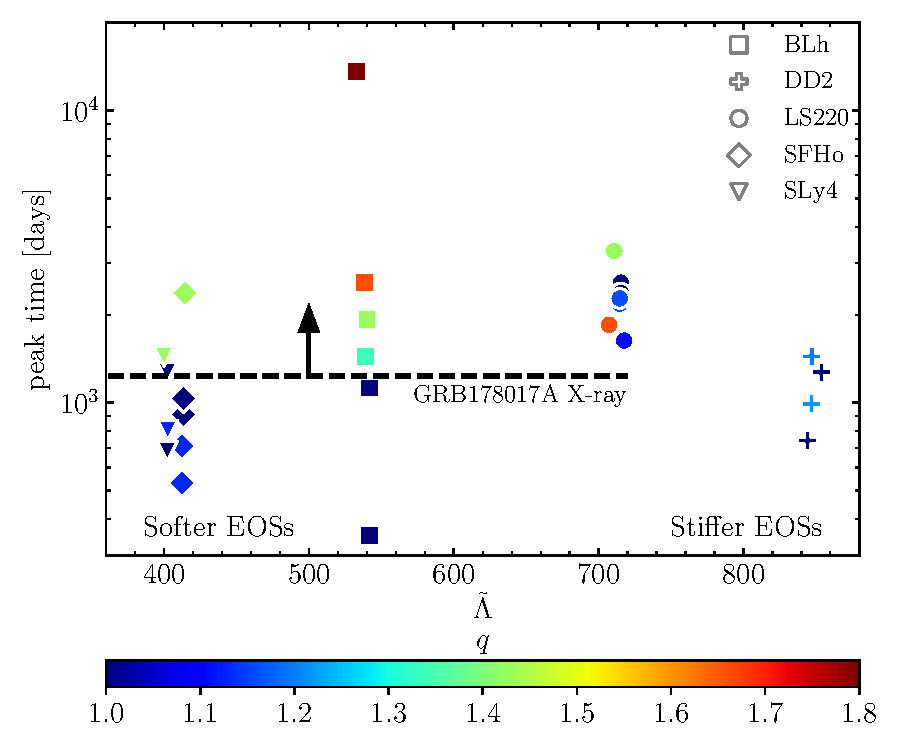
\includegraphics[height=5cm]{phd_figs/kn_afterglow/scatter_lightcurve_tpeak_vs_lambda.pdf}
    }};
}

\end{tikzpicture}

\end{frame}